%\subsection{Schema generale: definizione di un alert con estensioni}
%\begin{figure}[H]
%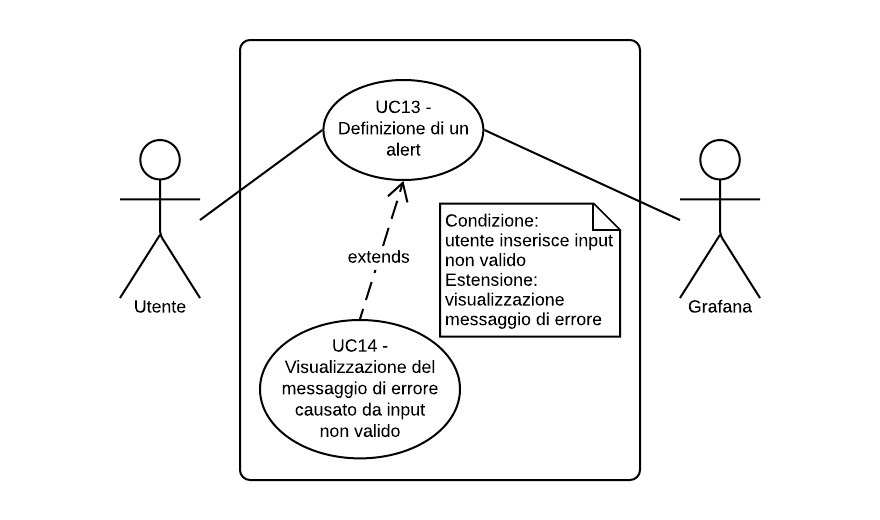
\includegraphics{img/UC13 - Schema generale.png}
%\caption{Schema generale: definizione di un alert con estensioni}
%\end{figure}
\subsection{UC13 - Definizione di un alert}
\begin{figure}[H]
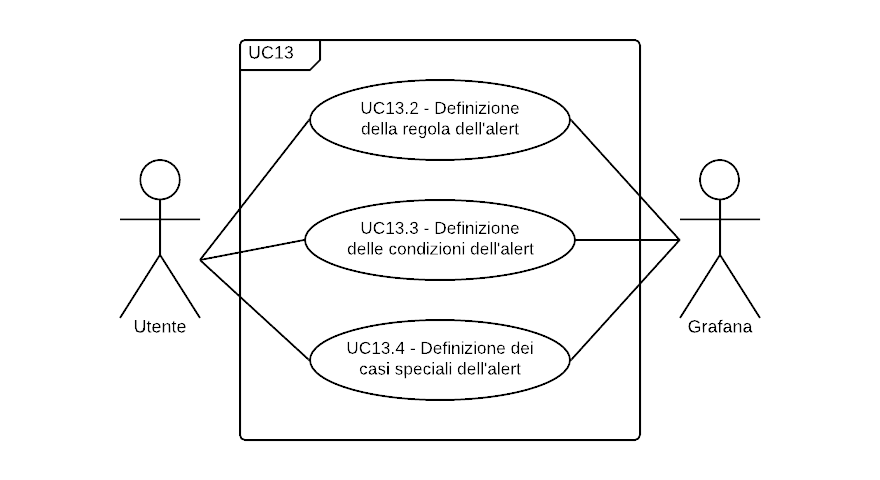
\includegraphics{img/UC13_-_Definizione_di_un_alert.png}
\caption{Diagramma degli use case di UC13}
\end{figure}
\begin{itemize}
	\item \textbf{Codice identificativo}: UC13;
	\item \textbf{Titolo}: definizione di un alert\glo;
	\item \textbf{Attore primario}: utente;
	\item \textbf{Attore secondario}: Grafana\glo;
	\item \textbf{Descrizione}: l'utente definisce un alert\glosp ovvero un elemento caratteristico di Grafana\glosp che rappresenta l'effetto del superamento di una soglia;
	\item \textbf{Precondizione}: l'utente è autenticato nel sistema software Grafana\glosp ed è presente una sua istanza, cloud o locale, su cui è stato aggiunto un pannello grafico che monitora una serie di dati;
	\item \textbf{Postcondizione}: viene inserito e definito con successo un alert\glosp nel pannello grafico scelto;
	\item \textbf{Scenario principale}: 
	\begin{enumerate}
		\item definizione della regola dell'alert\glosp (UC13.2);
		\item definizione delle condizioni dell'alert\glosp (UC13.3);
		\item definizione dei casi speciali dell'alert\glosp (UC13.4).
	\end{enumerate}
	\item \textbf{Estensioni}:	
	\begin{enumerate}
		\item visualizzazione del messaggio di errore causato da input non valido (UC13).
	\end{enumerate}
\end{itemize}

\subsubsection{UC13.2 - Definizione della regola di un alert}
\begin{itemize}
	\item \textbf{Codice identificativo}: UC13.2;
	\item \textbf{Titolo}: definizione della regola dell'alert\glo;
	\item \textbf{Attore primario}: utente;
	\item \textbf{Attore secondario}: Grafana\glo;
	\item \textbf{Descrizione}: l'utente definisce la regola principale di funzionamento dell'alert\glosp che comprende la scelta del nome, un valore che indica l'intervallo di tempo tra i controlli sui dati e un valore che indica per quanto tempo continuare il controllo;
	\item \textbf{Precondizione}: l'utente è autenticato nel sistema software Grafana\glosp ed è presente una istanza di Grafana\glosp cloud o locale su cui è stato aggiunto un pannello grafico che monitora una serie di dati;
	\item \textbf{Postcondizione}: l'utente ha definito la regola di funzionamento dell'alert\glo;
	\item \textbf{Scenario principale}: l'utente definisce le regole di funzionamento dell'alert\glosp inserendo nome e tempi di interrogazione.
\end{itemize}

\subsubsection{UC13.3 - Definizione delle condizioni di un alert}
\begin{itemize}
	\item \textbf{Codice identificativo}: UC13.3;
	\item \textbf{Titolo}: definizione delle condizioni dell'alert\glo;
	\item \textbf{Attore primario}: utente;
	\item \textbf{Attore secondario}: Grafana\glo;
	\item \textbf{Descrizione}: l'utente definisce le condizioni di funzionamento dell'alert\glo, cioè i limiti tali per cui, se superati, segnalano la presenza di dati oltre la soglia prestabilita nel pannello grafico;
	\item \textbf{Precondizione}: l'utente è autenticato nel sistema software Grafana\glosp ed è presente una sua istanza, cloud o locale, su cui è stato aggiunto un pannello grafico che monitora una serie di dati;
	\item \textbf{Postcondizione}: l'utente ha definito una o più condizioni dell'alert\glo;
	\item \textbf{Scenario principale}: l'utente definisce le condizioni di funzionamento dell'alert\glosp selezionando la funzione di aggregazione dati ed il valore soglia che attiva l'allarme.
\end{itemize}

\subsubsection{UC13.4 - Definizione dei casi speciali di un alert}
	\begin{itemize}
	\item \textbf{Codice identificativo}: UC13.4;
	\item \textbf{Titolo}: definizione dei casi speciali dell'alert\glo;
	\item \textbf{Attore primario}: utente;
	\item \textbf{Attore secondario}: Grafana\glo;
	\item \textbf{Descrizione}: l'utente definisce il comportamento dell'alert\glosp al verificarsi di situazioni particolari, come nel caso in cui non ci siano dati, siano tutti nulli, la richiesta va in timeout o c'è un errore di esecuzione;
	\item \textbf{Precondizione}: l'utente è autenticato nel sistema software Grafana\glosp ed è presente una sua istanza, cloud o locale, su cui è stato aggiunto un pannello grafico che monitora una serie di dati;
	\item \textbf{Postcondizione}: l'utente ha definito uno o più comportamenti speciali dell'alert\glo;
	\item \textbf{Scenario principale}: l'utente definisce i comportamenti speciali dell'alert\glosp nei casi particolari come assenza di dati o errori di esecuzione. Per farlo seleziona i comportamenti desiderati tramite il pannello fornito da Grafana\glo.
\end{itemize} 
